\section{Introduction} \label{sec:background}

Successful evolutionary search depends the production of heritable, novel phenotypic variation, some of which must not be severely deleterious.
Without any heritable variation --- or even just without any viable heritable variation --- evolution stagnates.
The capacity of a population to generate viable heritable phenotypic variation is referred to as evolvability.

Different evolving systems can exhibit different degrees of evolvability.
Different digital evolution systems exhibit different evolvability TODO
Natural systems, in particular, are thought to generally exhibit greater evolvability than digital evolution systems \cite{mengistu2016evolvability}.
Let us examine a pair of biological examples of non-arbitrary phenotypic outcomes under mutation to build our intuition for evolvability.

A developmental constraint against certain non-viable phenotypic variation in  \textit{Drosophilia melangoster} was discovered through artificial selection experiments \cite{coyne1987lack, tuinstra1990lack}.
In these experiments,  researchers were able to successfully select for bilaterally symmetric phenotypic criteria, such as overall smaller eyes, but were unable to successfully select for bilaterally asymmetric phenotypic traits, such as different-sized eyes.
Tuinstra et al. hypothesize that the very nature of the developmental process constrains the phenotypic variation that can be observed in offspring, in this case curtailing the abundance of offspring that lack bilateral symmetry.
Specifically, they hypothesize that a lack of bilateral symmetry-breaking information during the embryological development of *Drosophila* explains the negative result of artificial selection for bilaterally asymmetric phenotypic traits.
In this way, the distribution of phenotypic diversity in offspring is biased away from (likely non-viable) asymmetric variation.

In addition to qualities that constrain against non-viable mutational outcomes, biological organisms can possess qualities that facilitate significant heritable variation for a phenotypic trait.
Somatotropin, also known as growth hormone, is well known for its widespread anabolic effects on tissues throughout the body.
Mutations affecting the regulatory pathways that regulate somatotropin production and release, the receptors and cell signaling components that mediate cellular response to somatotropin, and the protein itself all provide avenues for significant heritable variation in body size \cite{devesa2016multiple}.
Dog breeds exhibit a range of body weights spanning nearly an entire order of magnitude.
Indeed, among certain groups of dogs, much of this variation can be explained by just six genes, several of which are associated with pathways somatotropin participates in \cite{rimbault2013derived}.
The presence of hormonal signaling pathways like those somatotropin participates in can be viewed as making a broad range of heritable phenotypic variation more readily realizable via mutation.

A general consensus exists in the literature that evolvability stems from traits that facilitate the generation of \textit{novel} heritable phenotypic variation that is \textit{viable} \cite{tarapore2015evolvability}.

[describe evolvability signature]
Tarapore et al. introduced an evolvability measure that attempts to take a more clear-eyed view of both of the primary aspects of evolvability: the amount of heritable variation among offspring and the fitness effects of that variation \cite{tarapore2015evolvability}.
They forgo use of a scalar metric to describe evolvability, instead reporting evolvability using what they term a ``signature.''
Essentially, the signature is a two-dimensional heatmap presenting the changes in phenotypic form and fitness observed in individual offspring from a single parent.
Normalized mutual information between the phenotypic states of parent and offspring is used to quantify the amount of change in phenotypic form observed in an offspring.
Proportion decrease in fitness is used to quantify the fitness difference between parent and offspring.
For a highly evolvable individual, we would expect to see offspring occurring with significant frequency in the corner of the heatmap indicating significant change in phenotypic form with slight or no loss of fitness.
The evolvability signature provides a nuanced snapshot of evolvability, allowing for interaction between the two primary components of evolvability to be visualized.
Such information can be highly diagnostic, for example alerting researchers to phenomena that might appear falsely promising using other metrics, such as genetic changes that alter phenotypic form significantly but at great cost to fitness or genetic changes that are beneficial to fitness but fail to uncover novel phenotypic form.
[ADD EXAMPLE READING IT FIGURE]

To rival that of natural systems
Evolvability is desirable in artificial evolution systems for practical ends --- developing more evolvable artificial evolution systems will allow evolutionary algorithms to tackle more sophisticated problems more effectively.
Understanding evolvability is also important to scientific ends for evolutionary biologists and evolutionary computing researchers alike  \cite{mengistu2016evolvability, pigliucci2008evolvability}.

\subsection{Genotype-Phenotype Map and Evolvability}

In biological science, a distinction is drawn between an organism's genotype and phenotype.
Phenotype refers to an organism's observable characteristics (morphological, behavioral, physiological, chemical, etc.) that govern its interaction with the environment and ultimately determine its fitness.
Genotype refers the heritable information that influences the phenotype displayed by the individual, i.e. the organism's DNA.
Development is the process through which an organism's genotype shapes (but does not completely determine due to environmental influence) its phenotype.
It is useful to abstract development as a mathematical function that takes genetic information as its input and outputs phenotypic characteristics.
This mathematical function representing development is referred to as the genotype-phenotype map \cite{alberch1991genes}.

The nature of the genotype-phenotype map employed in an evolving system is thought to influence that system's evolvability \cite{pigliucci2010genotype}.
Let us discuss three theoretical constructs that are useful to understanding the relationship between the genotype-phenotype map and evolvability: latent evolvability, acquired evolvability, and innate evolvability.

The terms latent evolvability and acquired evolvability were introduced by Reisinger et al. in \cite{reisinger2005towards} to discuss canalization, the ability of a population to bias the types of phenotypic variability generated among its offspring in order to exploit fitness biases specific to its environment.
It is key to observe that canalization is a ``learned'' bias, developed over the course of evolution in response to selection pressure in a particular environment \cite{reisinger2005towards}.
Latent evolvability describes a genotype-phenotype map's potential to exhibit canalization while acquired evolvability describes actual canalization exhibited by an evolving population in response to a particular fitness environment.
I introduce the term innate evolvability to describe bias towards viable variation that is inherent to a genotype-phenotype map.
For example, Clune et al. identify bias towards phenotypic regularity, which in certain environments tends to be a useful trait, as an inherent quality of indirect genetic encoding \cite{clune2008generative}.

Innate, latent, and acquired evolvability all provide opportunities for intervention  by digital evolution researchers to get evolvable genotype-phenotype mapping.
1) latent --- design an encoding \cite{reisinger2005towards},
2) acquired --- use selection to try to get here (i.e. evolvability selection, modularly varying environments, etc.) \cite{mengistu2016evolvability, kashtan2005spontaneous} (relies on genotype-phenotype map exhibiting innate evolvability)
3) innate --- design an encoding \cite{clune2011performance}.


Hand-designing genotype-phenotype mappings that exhibit latent evolvability and innate evolvability is
1) hard
2) problem-specific

+ evolvable G-P maps
  + It is of theoretical interest to study genotype-phenotype maps and their relation to evolvable and practical interest to be able to work with them: more evolvable G-P maps enables more sophisticated digital evolution.
  + manual design \cite[p 223]{downing2015intelligence}
  "artificial evolutionary developmental systems have yet to achieve convincing success on anything beyond quite simple tasks... finding effective developmental recipes for growing complex physical structures and control systems has proven to be an extremely daunting task... Researchers always return to the same question: What aspects of natural development can actually contribute to improving artificial design, rather than being merely scientifically interesting to implement?"
  + evolve them \cite{reisinger2007acquiring}



  In fact, the distinction can become blurred in the realm of evolutionary algorithms, where the phenotypic characteristics of an individual might be directly encoded in the genotype.


  Hand-design of genotype-phenotype maps is common practice in evolutionary computing.
  These genotype-phenotype mappings, such as HyperNEAT, have been used with good success and studied extensively \cite{stanley2009hypercube, woolley2010evolving, clune2011performance}.
  In particular, there has been interest in designing dynamic genotype-phenotype mappings that are influenced by the contents of a genome, as occurs in nature, so that an evolvable mapping may themselves be evolved \cite{reisinger2007acquiring}.
  Nonetheless, existing genotype-phenotype mappings can be domain-specific;
  a scheme useful for artificial neuroevolution, for example, likely isn't useful in a linear genetic programming context.


\subsection{Evolution and Learning}

I propose a propose a third way: directly learn an evolvable genotype-phenotype mapping using machine learning techniques for unsupervised learning.
This idea is inspired by the notion that natural evolution learns to generalize \cite{kouvaris2017evolution} \cite{watson2016can}

he question thus arises: is evolution by natural selection (e.g., by adapting the organization of developmental processes) able to facilitate subsequent adaptation in the same way that a learning system can exploit knowledge from past experience? If so, evolution might be a ‘smarter’ problem solver than generally appreciated and learning theory could explain how. \cite{watson2016can}

A potential resolution is provided by the idea that evolution may discover and exploit information not only about the particular phenotypes selected in the past, but their underlying structural regularities: new phenotypes, with the same underlying regularities, but novel particulars, may then be useful in new environments. \cite{kouvaris2017evolution}

We support the conclusion that evolving systems and learning systems are different instantiations of the same algorithmic principles by showing that existing results from the learning domain can be transferred to the evolution domain \cite{kouvaris2017evolution}

This paper proposes a different take on automatic generation of evolvable genotype-phenotype mapping by proposing two techniques to directly learn evolvable genotype-phenotype mappings through artificial neural network autoencoders.
It is hoped that this project will yield useful evolutionary computing methodology to achieve automatic design of highly evolvable genotype-phenotype mappings.

\subsection{Autoencoder Neural Networks}

The two proposed genotype-phenotype map learning techniques are based on artificial neural network autoencoders.
These are networks that are trained to regurgitate as output the input that they were provided.
Such networks are used to discover efficient lower-dimensional codings for datasets and, more recently, as method for generative modeling \cite{liou2014autoencoder, kingma2013auto}.


\begin{figure}
  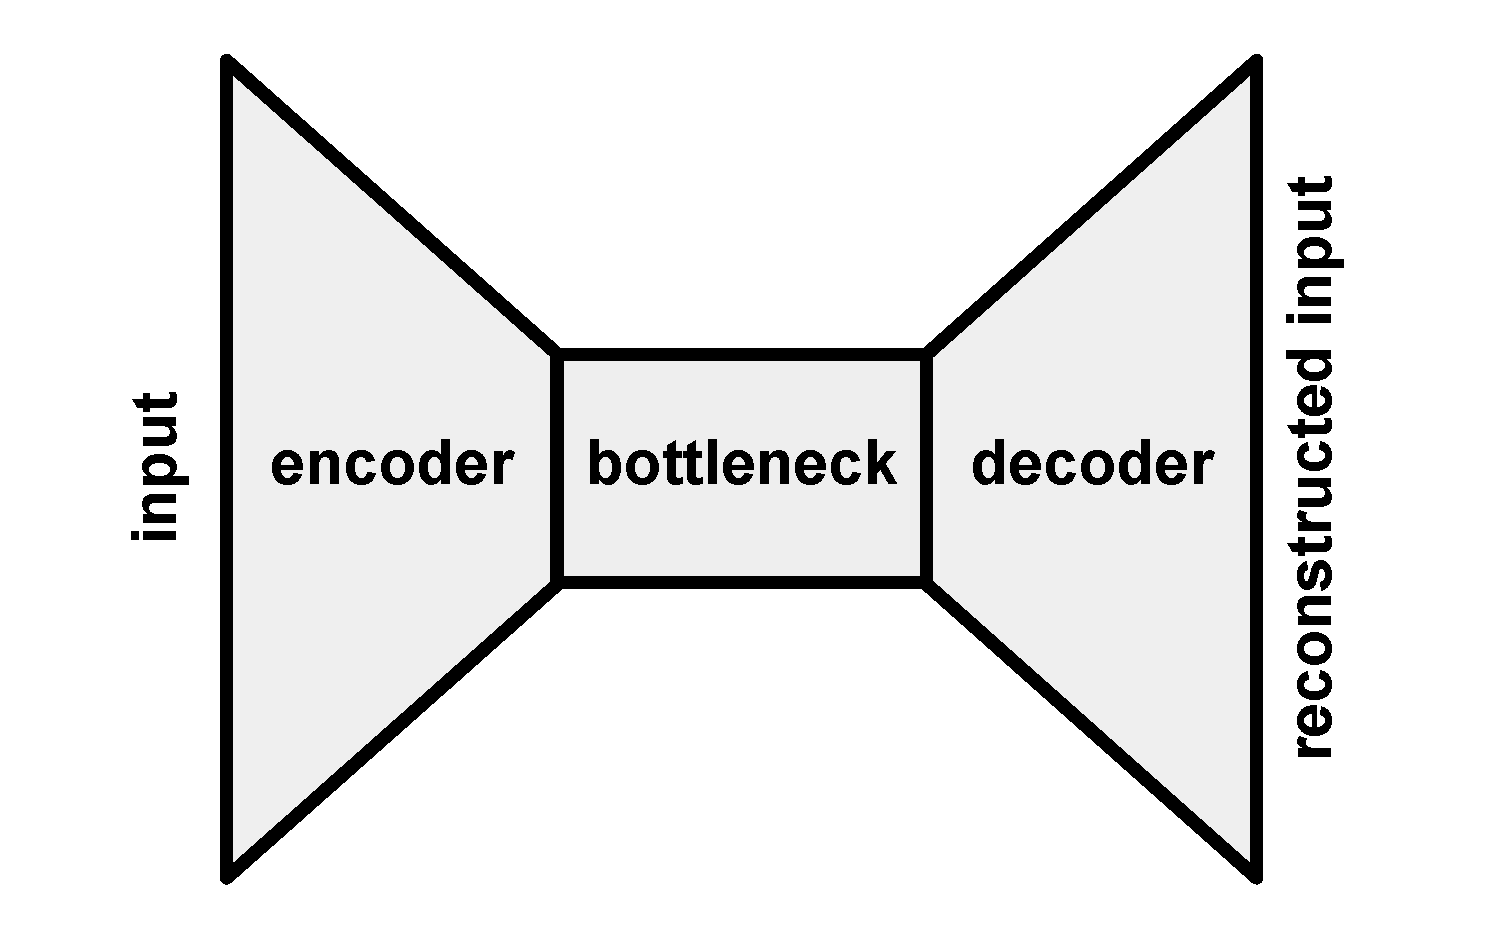
\includegraphics[width=0.5\linewidth]{img/bottleneck}
  \caption{Schematic of a bottlenecked autoencoder.}
  \label{fig:bottleneck}
\end{figure}


The first technique uses a bottlenecked autoencoder.
Figure \ref{fig:bottleneck} provides a schematic impression of such an autoencoder.
This autoencoder has a small layer in the middle that information must pass through to reach the output.
Thus, the autoencoder is forced to learn a compact representation for the input it is trained with that can pass through the bottleneck.
The part of the autoencoder that precedes the bottleneck is called the encoder and the part that follows is called the decoder.
This autoencoder will be trained to encode phenotypes taken from fitness peaks throughout an evolutionary search space.
The idea of this approach is that, because the bottleneck provides a compact representation of those high-fitness phenotypes, using the decoder as a genotype-phenotype mapping will readily allow mutation to move the phenotype between otherwise distant fitness peaks.

\begin{figure}
  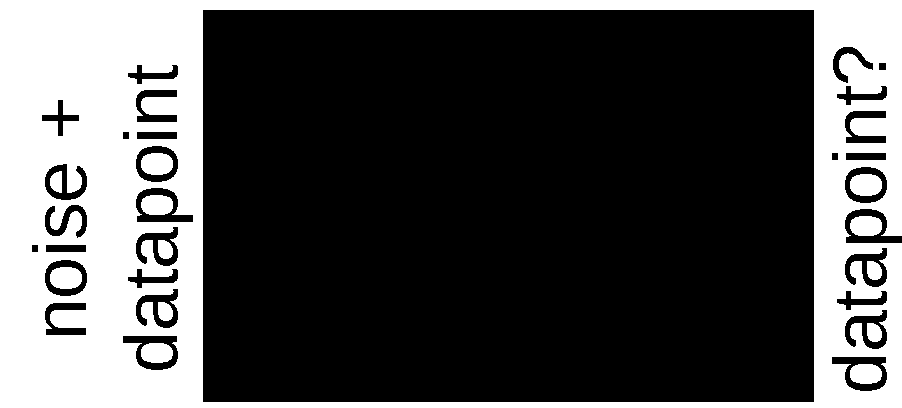
\includegraphics[width=\linewidth]{img/denoiser}
  \caption{
    Schematic of a denoising autoencoder.
  }\label{fig:denoiser}
\end{figure}


The second technique uses a denoising autoencoder.
Figure \ref{fig:denoiser} provides a schematic depiction of such an autoencoder.
These autoencoders have not bottleneck.
Instead, they are trained to reconstruct noisy input into its original unadulterated form.
This autoencoder will be trained to reconstruct phenotypes taken from fitness peaks throughout an evolutionary search space.
For this approach, the entire denoising autoencoder would be used as the genotype-phenotype mapping.
The idea of this design is that mutations that would otherwise be deleterious will effectively be interpreted as noise and prevented from being expressed by the genotype-phenotype mapping.
Effectively, this mapping should flatten out the valleys between local fitness peaks to allow evolution to more readily drift between those local fitness peaks.


\subsection{Learning an Evolvable Genotype-Phenotype Mapping}
